\documentclass{stdlocal}
\begin{document}
\section{Background} % (fold)
\label{sec:background}
  % virtual subsection Introduction
  To systematically approach the implementation of PRNGs, basic knowledge in the topics of stochastics and finite fields is administrable.
  Together, these topics will give a deeper understanding of randomness in deterministic computer systems, a formal description of pseudorandom sequences and generators, and the mathematical foundation of Monte Carlo algorithms.
  Based on them, we are capable of scientifically analyzing PRNGs concerning their randomness properties.
  Vectorization techniques can be conceptualized by the architecture of modern SIMD-capable multiprocessors and their instruction sets.
  Especially the knowledge of typical instructions will make the design of a new API and its application to Monte Carlo simulations clear.
  The following sections will give an overview of the named topics.

  \subsection{Mathematical Preliminaries} % (fold)
  \label{sub:mathematical_preliminaries}
    \subsubsection{Probability Theory} % (fold)
    \label{ssub:stochastics}
      The observation of random experiments resulted in the construction of probability theory.
      But probability theory itself does not use a further formalized concept of randomness \autocite{schmidt2009}.
      % Randomness itself plays a minor role in probability theory and is used in form of realizations of random variables.
      In fact, it allows us to observe randomness without defining it \autocite{volchan2002}.
      % Actually, typical formalizations rely on probability theory.
      % This connection makes the development of RNGs possible.
      % Hence, in the following we will give only the formal definition of relevant structures without further discussions and will postpone an examination of randomness to the next subsection.
      Hence, we will postpone an examination of truly random sequences to the next section.

      According to \textcite{schmidt2009}, Kolmogorov embedded probability theory in the theory of measure and integration.
      Albeit it heavily relies on measure-theoretical structures, probability theory is one of the most important applications of measure and integration theory.
      Therefore we will assume basic knowledge in this topic and refer to \textcite{schmidt2009} and \textcite{elstrodt2011} for a more detailed introduction to measure spaces, measurable functions, and integrals.
      Propositions and theorems will be given without proof.

      The underlying structure of probability theory, which connects it to measure theory, is the probability space.
      It is a measure space with a finite and normalized measure.
      This gives access to all the usual results of measure theory and furthermore unifies discrete and continuous distributions.
      \autocite[p.~193~ff.]{schmidt2009}

      \begin{definition}[Probability Space]
        A probability space is a measure space $\roundBrackets{\Omega, \mathscr{F}, P}$ such that $P(\Omega)=1$.
        In this case, we call $P$ the probability measure, $\mathscr{F}$ the set of all events, and $\Omega$ the set of all possible outcomes of a random experiment.
      \end{definition}
      % For our purposes, the set of possible outcomes $\Omega$ will be a finite or countable infinite set.
      % Hence, we can choose $\mathscr{F}$ to be the power set $\mathscr{P}(\Omega)$.
      Due to the complex definition of a measure space, it is convenient to not have to explicitly specify the probability space when analyzing random experiments.
      Instead, we use random variables which are essentially measurable functions on a probability space \autocite[p.~194]{schmidt2009}.
      For complicated cases, these will serve as observables for specific properties and will make the analysis much more intuitive.

      \begin{definition}[Random Variable]
        Let $(\Omega,\mathscr{F},P)$ be a probability space and $(\Sigma,\mathscr{A})$ a measurable space.
        A measurable function $\function{X}{\Omega}{\Sigma}$ is called a random variable.

        In this case, we denote with $P_X\define P\composition\inverse{X}$ the distribution and with $(\Sigma,\mathscr{A},P_X)$ the probability space of $X$.
        % We call $X(ω)$ for $ω\in\Omega$ a realization of $X$.
        % Let $\function{Y}{\Omega}{\Sigma}$ be another random variable.
        % $X$ and $Y$ are identically distributed if $P_X = P_Y$.
        Two random variables are identically distributed if they have the same distribution.
        Additionally, we say that $X$ is a real-valued random variable if $\Sigma = \setReal$ and $\mathscr{A} = \mathscr{B}(\setReal)$.
      \end{definition}
      From now on, if a random variable is defined then, if not stated otherwise, it is assumed there exists a proper probability space $(\Omega,\mathscr{F},P)$ and measurable space $(\Sigma, \mathscr{A})$.

      Another important concept of stochastics is known as independence.
      In \textcite{schmidt2009} it is defined for a family of events, a family of sets of events, and a family of random variables.
      If we think of random variables as observables then their independence means that their outcomes do not influence each other.
      % It makes only sense in the context of probability theory
      For our purposes, the general definition of all three forms of independence is distracting.
      In a computer, it makes no sense to talk about infinite sequences.
      Therefore the following definition of independence takes only a finite sequence of random variables into account.
      Furthermore, to make it more understandable, this definition uses a theorem from \textcite[p.~238]{schmidt2009} which characterizes the independence of random variables.
      % Here, we will use a simpler equivalent definition  because, for a computer, all we need are finite sequences of random variables.

      \begin{definition}[Independence]
        % Let $(\Omega,\mathscr{F},P)$ be a probability space.
        % Two events $A, B \in \mathscr{F}$ are independent if $P(A\cap B)=P(A)P(B)$.
        % Let $(\Sigma_i,\mathscr{A}_i)$ for $i\in\set{1,2}{}$ be measurable spaces and $X_i$ random variables with $X\define X_1\times X_2$.
        % They are called independent if $P_X = P_{X_1} \otimes P_{X_2}$.
        Let $n\in\setNatural$ and $X_i$ be a random variable for all $i\in\setNatural$ with $i\leq n$.
        We denote the respective random vector with $X \define \roundBrackets{X_i}_{i=1}^n$.
        Then these random variables are independent if the following equation holds.
        \[
          P_X = \bigotimes_{i=1}^n P_{X_i}
        \]
      \end{definition}
      Typical observations of random sequences include the estimation of the expectation value and the variance.
      Both of these values are needed for analyzing PRNGs and the development of Monte Carlo simulations \autocite[p.~30~ff.]{landau2014}.
      Due to their deep connection to the integral, both of these moments are defined for real-valued random variables.
      We give the usual definitions based on \textcite[p.~274~ff.]{schmidt2009} in a simplified form.

      \begin{definition}[Expectation Value and Variance]
        Let $X$ be a real-valued random variable such that $\integral{\Omega}{}{\absolute{X}}{P}<\infty$.
        Then the expectation value $\expect X$ and variance $\var X$ of $X$ is defined in the following way.
        \[
          \expect X \define \integral{\Omega}{}{X(ω)}{P(ω)}
          \separate
          \var X \define \expect\roundBrackets{X - \expect X}^2
        \]
      \end{definition}
      To not rely on the underlying probability space directly, we want to be able to compute the expectation value through the respective distribution of the random variable.
      The theory of measure and integration gives the following proposition, also known as rule of substitution \autocite[p.~276]{schmidt2009}.

      \begin{proposition}[Substitution]
        Let $X$ be real-valued random variable and $\function{f}{\setReal}{\setReal}$ a measurable function such that $\integral{\Omega}{}{\absolute{f}}{P_X} < \infty$.
        Then the following equation holds.
        \[
          \expect(f\composition X) = \integral{\setReal}{}{f(x)}{P_X(x)}
        \]
        In particular, if $\expect \absolute{X} < \infty$ then the above equation can be reformulated as follows.
        \[
          \expect X = \integral{\setReal}{}{x}{P_X(x)}
        \]
      \end{proposition}
      The distribution of real-valued random variables is univariate and as a result can be described by so-called cumulative distribution functions (CDFs).
      The CDF intuitively characterizes the distribution and simplifies the analysis.
      Further, it can be proven that every CDF belongs to a univariate distribution.
      According to \textcite[p.~246]{schmidt2009}, this is the theorem of correspondence.
      Sometimes it is even possible to define a probability density; a function that is the Lebesgue density of the respective distribution \autocite[p.~255]{schmidt2009}.

      \begin{definition}[Probability Density and Cumulative Distribution Function]
        Let $X$ be a real-valued random variable.
        Then the respective cumulative distribution function is defined as follows.
        \[
          \function{F_X}{\setReal}{[0,1]}
          \separate
          F_X(x) \define P_X((-\infty,x])
        \]
        We call the function $\function{p}{\setReal}{[0,\infty)}$ a probability density of $X$ if for all $A\in\mathscr{B}(\setReal)$
        \[
          P_X(A) = \integral{A}{}{p(x)}{λ(x)}\ .
        \]
      \end{definition}
      % \begin{theorem}[Correspondence]
      %   Let $X$ be a real-valued random variable.
      %   There exists a unique monotone non-decreasing, right-continuous function $\function{F_X}{\setReal}{[0,1]}$ with
      %   \[
      %     \lim_{x\rightarrow -\infty} F_X(x) = 0
      %     \separate
      %     \lim_{x\rightarrow +\infty} F_X(x) = 1
      %   \]
      %   such that
      %   \[
      %     P_X((a,b]) = F(b) - F(a)
      %   \]
      % \end{theorem}
      As well as CDFs, probability densities can greatly simplify computations which are based on absolute continuous random variables.
      The following proposition, obtained from \textcite{schmidt2009}, shows the simplified computation of an expectation value through a Lebesgue integral.

      \begin{proposition}[Chaining]
        Let $X$ be a real-valued random variable with $p$ as its probability density.
        If $\function{f}{\setReal}{\setReal}$ is a measurable function such that $\expect \absolute{f\circ X} < \infty$ then
        \[
          \expect \roundBrackets{f\composition X} = \integral{\setReal}{}{f(x)p(x)}{λ(x)}\ .
        \]
      \end{proposition}
      A last important theorem to name is the strong law of large numbers (SLLN).
      According to \textcite[p.~13]{graham2013}, the principles of Monte Carlo methods are based on this theorem.
      Please note, there exist many more variations of this theorem.
      We will again use a simplified version from \textcite{graham2013}.

      \begin{theorem}[Strong Law of Large Numbers]
        Let $(X_n)_{n\in\setNatural}$ be a sequence of iid real-valued random variables with finite expectation value $μ$.
        Then the following equation holds $P$-almost everywhere.
        \[
          \lim_{n\to\infty} \frac{1}{n}\sum_{i=1}^n X_i = μ
        \]
      \end{theorem}
    % subsubsection stochastics (end)

    % \subsubsection{Finite Fields} % (fold)
    % \label{ssub:finite_fields}

    % subsubsection finite_fields (end)
  % subsection mathematical_preliminaries (end)

  \subsection{Pseudorandom Number Generators} % (fold)
  \label{sub:pseudorandom_number_generators}

    \subsubsection{Random Sequences}
    In the above subsection \ref{sub:mathematical_preliminaries} the theory of probability was introduced to make an examination of randomness possible.
    Randomness is a difficult concept and drives many philosophical discussions.
    According to \textcite{volchan2002} and \textcite[\ppno~10-11]{kneusel2018}, humans have a bad intuition concerning the outcome of random experiments.
    But for our purposes, it would suffice to find a formal mathematical definition applicable to RNGs.
    However, such a formal concept, which is also widely accepted and unique, has not been found yet \autocite{volchan2002}.

    The first problem about randomness is the word itself.
    It is unclear and vague because there is no intentional application.
    To be more specific, we will observe randomness in form of random sequences of real numbers.
    But as stated in \textcite{volchan2002} the question if a sequence is random decides at infinity.
    As long as we are only observing finite sequences, we cannot decide if such a sequence is the outcome of a truly random experiment or the result of a non-random algorithm.
    Following his explanation, \citeauthor{volchan2002} makes clear that typical characterizations of a random sequence are closely associated with noncomputability.
    So even if we would be able to algorithmically produce an infinite amount of numbers, the resulting sequence could not be seen as truly random.
    A modified version of this idea which is easier to understand is given in \textcite{kneusel2018}, where a sequence of values $(x_n)_{n\in\setNatural}$ is truly random if there exists no algorithm such that for all $n\in\setNatural$ the value $x_{n+1}$ can be computed as a function of all $x_i$ with $i\in\setNatural$ and $i\leq n$.
    Put more simply, knowing finitely many elements of a truly random sequence does not enable us to predict the next values within a computer.
    Furthermore, the question if a sequence is random cannot be decided by an algorithm.
    Hence, the existing formal concepts for truly random sequences are not applicable to computer systems.
    Instead, \citeauthor{volchan2002} proposed a more pragmatic principle: \textquote[\cite{volchan2002}]{if it acts randomly, it is random} --- the use of pseudorandom sequences.

    % As a result, we will not use a formalized concept of randomness.
    A computer is only capable of using finite sequences of values and for the development of RNGs, it is enough to measure and compare different properties of truly random sequences to a sequence of real numbers.
    For this, we rely on probability theory and first define an abstract random sequence drawn from a random experiment.
    The definition will use realizations of random variables to model the samples of a random experiment.
    We make sure that these variables are identically and independent distributed (iid).
    This makes analyzing other sequences simpler and imposes no boundary because every important distribution can be generated out of iid random variables \autocite[\ppno~81-111]{kneusel2018}.

    \begin{definition}[Random Sequence]
      Let $I$ be a countable index set and $(X_n)_{n\in I}$ be a sequence of iid real-valued random variables.
      Then a realization of $(X_n)_{n\in I}$ is called a random sequence.
    \end{definition}
    % A system which generates an arbitrarily long abstract random sequence is called a true random number generator (TRNG).
    Generating a truly random sequence in a deterministic computer system is impossible.
    An RNG which is able to generate such a sequence is called a true random number generator (TRNG) and is typically implemented as a device drawing random samples from an essentially non-deterministic physical process, like temperature fluctuations \autocite{intel-drng}.
    % subsubsection random_and_pseudorandom_sequences (end)

    % \subsubsection{Random and Pseudorandom Number Generators} % (fold)
    % \label{ssub:random_and_pseudorandom_number_generators}
    \subsubsection{Pseudorandom Sequences}
    The given abstract definition of a random sequence in terms of probability theory helps to assess the randomness properties of a given sequence produced by a computer.
    Typically, a computer-generated sequence which fulfills various conditions about randomness will be called a pseudorandom sequence.
    The respective structure and algorithm which produced the sequence is then called a PRNG.

    For computer programming and simulations, the usage of a TRNG would introduce severe disadvantages in contrast to a PRNG.
    Concerning program verification, debugging, and the comparison of similar systems, the reproducibility of results is essential \autocite{lecuyer2015}.
    A truly random sequence produced by physical devices, such as thermal noise diodes or photon trajectory detectors, is not reproducible and can therefore not be conveniently used for mathematical and physical simulations \autocite{lecuyer2015}.
    According to \textcite{lecuyer2015}, a given simulation should produce the same results on different architectures for every run.
    This property becomes even more important if parallel generation of random numbers with multiple streams is taken into account.
    Additionally, considering the performance of random number generation PRNGs tend to be much faster than TRNGs \autocite{intel-drng}.
    Thus, especially for Monte Carlo methods, PRNGs are a key resource for computer-generated random numbers \autocite{bauke2007}.

    For a detailed discussion about its mathematical properties, design, and implementation, the concept of a PRNG has to be formalized.
    In this thesis, we use the following slightly modified variation of \citeauthor{lecuyer1994}'s definition \autocite{lecuyer1994,lecuyer2015,barash2017,bauke2007}.
    It assumes a finite set of states and a transition function which advances the current state of the PRNG by a recurrence relation.
    For the output, a finite set of output symbols and a generator function which maps states to output symbols is chosen.
    As of \textcite{bauke2007}, almost all PRNGs produce a sequence of numbers by a recurrence.
    Hence, the given formalization is widely accepted and builds the basis for further discussions about pseudorandom numbers \autocite{lecuyer1994,lecuyer2015,barash2017,bauke2007}.

    \begin{definition}[Pseudorandom Number Generator]
      Let $\mathscr{G}\define (S,T,U,G)$ be a tuple consisting of a non-empty, finite set of states $S$, a transition function $\function{T}{S}{S}$, a non-empty, finite set of output symbols $U$ and an output function $\function{G}{S}{U}$.
      In this case $\mathscr{G}$ is called a PRNG.
    \end{definition}
    Given a PRNG and a seed value as an initial state, producing a sequence of pseudorandom numbers can be done by periodically applying the transition function on the current state and then extracting the output through the generator function \autocite{barash2017,lecuyer1994,lecuyer2015}.
    Here, we will use this method as the generalization of a pseudorandom sequence.
    Figure \ref{fig:scheme-pseudorandom-sequence} shows this process schematically.

    \begin{definition}[Pseudorandom Sequence of PRNG]
      Let $\mathscr{G}\define (S,T,U,G)$ be a PRNG and $s_0\in S$ be the initial state, also called the seed value.
      The respective sequence of states $(s_n)_{n\in\setNatural}$ in $S$ is given by the following equation for all $n\in\setNatural$.
      \[
        s_{n+1} \define T(s_n)
      \]
      The sequence $(u_n)_{n\in\setNatural}$ in $U$ given by the following expression for all $n\in\setNatural$ is then called the respective pseudorandom sequence of $\mathscr{G}$ with seed $s_0$.
      \[
        u_n \define G(s_n)
      \]
    \end{definition}
    \begin{figure}
      \center
      \begin{minipage}[b]{0.5\textwidth}
      \begin{alignat*}{3}
        s_0 \xrightarrow{T} &s_1 \xrightarrow{T} &&s_2 \xrightarrow{T} &&\ldots \\
        G &\downarrow &&\downarrow \\
        &u_1 &&u_2 &&\ldots
      \end{alignat*}
      \end{minipage}
      \caption[Generation of a Pseudorandom Sequence]{%
        The figure shows a scheme about the generation of a pseudorandom sequence for a given PRNG $\mathscr{G}\define (S,T,U,G)$ and seed value $s_0\in S$.
        The internal state is advanced by the transition function $T$ through a recurrence relation.
        To get an output value for the pseudorandom sequence the generator function $G$ is used.
      }
      \label{fig:scheme-pseudorandom-sequence}
    \end{figure}
    In the definition we have used a recursive formulation.
    For theoretical discussions and the initialization of multiple streams of pseudorandom numbers an explicit variation seems to be more adequate.
    The following lemma will be given without a proof, but it can be shown by mathematical induction.

    \begin{lemma}[Explicit Formulation of Pseudorandom Sequence]
    \label{lemma:explicit-formulation-pseudorandom-sequence}
      Let $\mathscr{G}\define (S,T,U,G)$ be a PRNG and $s_0\in S$ its initial state.
      Then the respective pseudorandom sequence $(u_n)_{n\in\setNatural}$ is given by the following formula for all $n\in\setNatural$.
      \[
        u_n = G\circ T^{n}(s_0)
      \]
    \end{lemma}

    \subsubsection{Explanation of the Concept}
    Using a TRNG in a computer system is like consulting an oracle \autocite{mueller2012}.
    We are calling a function with no arguments which returns a different value for every call.
    Let $(u_n)_{n\in\setNatural}$ be the respective pseudorandom sequence of a PRNG $\mathscr{G}$ with a given seed.
    Then in a computer $\mathscr{G}$ can be interpreted as a function with no parameters which produces the pseudorandom sequence $(u_n)_{n\in\setNatural}$ in the following way.
    Hereby, we understand $\leftarrow$ as the assignment operator that assigns a value given on the right-hand side to the variable given on the left-hand side.
    \[
      u_1 \leftarrow \mathscr{G}()
      \separate
      u_2 \leftarrow \mathscr{G}()
      \separate
      u_3 \leftarrow \mathscr{G}()
      \separate
      \ldots
    \]
    A PRNG has to artificially model this behavior by an internal state.
    Every function call must change this state according to the transition function.
    Consequently, if a PRNG should be used as an oracle in that sense, the set of states and the transition function in its definition are obligatory.

    It will be shown that the number of different states a PRNG can reach greatly affects the randomness of a respective pseudorandom sequence.
    A larger set of states is not a guarantee that the output of a PRNG will look more like a truly random sequence, but at least gives the opportunity to better mask its deterministic nature \autocite{oneill2014}.
    Therefore the number of states in general is much bigger than the number of different outputs.
    Through the usage of output symbols together with a generator function a PRNG can take advantage of a large set of states while returning only a few different values.
    This idea has two important implications.
    A generator function which shrinks the set of states to a smaller space of output symbols makes the PRNG less predictable and more secure \autocite{oneill2014}.
    The generator function would not be bijective and as a result we as consumers would not be able to draw conclusions about the current state of the PRNG based on its given output.
    Both properties are highly appreciated because they mimic the behavior of TRNGs.
    Hence, the set of output symbols and the generator function in the definition of PRNGs is as important as the set of states and the transition function.

    In the majority of cases, the transition function $T$ of a PRNG $\mathscr{G}$ should be injective \autocite{lecuyer1994,lecuyer2015,widynski2019,oneill2014}.
    Because we have a finite set of states this is equivalent to the proposition that $T$ is a permutation and therefore bijective \autocite[\ppno~201-202]{waldmann2017}.
    The property makes sure that every state is reached at a certain point in a sequence without introducing bias in the resulting distribution \autocite{oneill2014}.
    The generator function $G$ cannot be a permutation but should not distort the distribution either.
    Hence, a uniform function which maps to every output value the same number of input values is a perfect candidate \autocite{oneill2014}.

    \subsubsection{Randomization}
    The goal of PRNGs is to imitate the properties of TRNGs as much as possible \autocite{lecuyer1994} and at the same time retaining executability by a computer system and reproducibility for a given seed \autocite{lecuyer2015}.
    These restrictions make a pseudorandom sequence completely predictable and characterizable by its seed.
    So up until now, we have not introduced any kind of randomness to the definition of a PRNG.
    But to extend the process of generating a pseudorandom sequence with true randomness, the seed will be chosen to be a truly random number produced by a TRNG.
    \textcite{lecuyer1994} states that receiving such a seed is much less work and more reasonable than acquiring a long sequence of truly random values.
    A generator with a truly random seed can be seen as an extensor of randomness.
    Even today, \citeauthor{intel-drng} uses hardware-implemented PRNGs repeatedly seeded by a high-quality entropy source in their CPUs to provide a high-performance hardware module for producing random numbers with good statistical quality and protection against attacks \autocite{intel-drng}.

    \begin{definition}[Randomized Pseudorandom Sequence]
      Let $\mathscr{G}\define (S,T,U,G)$ be a PRNG and $X$ be an $S$-valued random variable with distribution $P_X$.
      Then the randomized pseudorandom sequence $(X_n)_{n\in\setNatural}$ of $\mathscr{G}$ with respect to $P_X$ is defined by the following expression for all $n\in\setNatural$.
      \[
        X_n \define G \circ T^n \circ X
      \]
    \end{definition}
    As with abstract random sequences, a truly random seed value is again modeled by a realization of the random variable $X$.
    As a result, the randomized pseudorandom sequence becomes a sequence of random variables which all depend on $X$.
    For the definition the explicit formulation in Lemma \ref{lemma:explicit-formulation-pseudorandom-sequence} was used.
    Typically, the distribution of seed values $P_X$ is chosen so that it is uniformly distributed in a certain subset of $S$ \autocite{matsumoto1998,oneill2014,lecuyer1994,lecuyer2015,bauke2007}.
    This makes sure that no bias will be introduced by the randomization.

    \subsubsection{Limitations and Mathematical Properties}
    As was already discussed, PRNGs have certain advantages in comparison with TRNGs.
    But they are also yielding essential and intrinsic limitations.
    From the previous paragraph, it becomes clear that all the samples of a randomized pseudorandom sequence are not stochastically independent.
    In general, this means the output of a PRNG can consist of certain regular patterns or artifacts \autocite{lecuyer1994,oneill2014}.
    In \textcite{lecuyer1994} these artifacts are also called the lattice structure.
    % Such patterns can be visualized by so-called randograms.
    % The typical approach to prevent the user of a PRNG to observe this dependence is to construct a complex generator function that scrambles the output.
    For applications that are using a large amount of random numbers, such patterns will introduce bias in the evaluated outputs.
    Hence, we will discuss a few mathematical properties a PRNG should fulfill to reduce the lattice structure as much as possible.

    \paragraph{Periodicity}
    Since the set of states in a PRNG is finite, every respective pseudorandom sequence has to be periodic or ultimately periodic \autocite{lecuyer1994,bauke2007}.
    First, a rigorous definition of this concept should be given.

    \begin{definition}[Periodic and Ultimately Periodic Sequences]
      Let $U$ be a non-empty set and $(u_n)_{n\in\setNatural}$ be a sequence in $U$.
      Assume there exist $ρ,τ\in\setNatural$ such that for all $n\in\setNatural_0$ the following holds.
      \[
        u_{τ+n+ρ} = u_{τ+n}
      \]
      Then $(u_n)$ is called ultimately periodic.
      The smallest possible values for ρ and τ, such that the equation holds, are called period and transient respectively.
       % with period ρ and transient τ.
      In particular, if τ equals to $1$ we call $(u_n)$ periodic with period ρ.
    \end{definition}
    This means an ultimately periodic sequence will be periodic after it reached its transient.
    Every periodic sequence is therefore ultimately periodic but not vice versa and as another consequence, the given concept is more general than the typical one of a periodic sequence.
    Please note that the values for ρ and τ are not unique.
    Let $ρ^*$ be the period and $τ^*$ be the transient.
    Then the equation given in the above definition holds for all values ρ and τ with respect to $m\in\setNatural$ and $n\in\setNatural_0$ in the following sense.
    \[
      ρ = mρ^*
      \separate
      τ = τ^* + n
    \]
    Choosing the minimal values allows us to talk about a unique transient and a unique period.
    In the following lemma we show the application of the definition to pseudorandom sequences.

    \begin{lemma}[Pseudorandom Sequences are Ultimately Periodic]
      Let $\mathscr{G}\define (S,T,U,G)$ be a PRNG and $s_0\in S$ its initial state.
      Then the respective pseudorandom sequence $(u_n)_{n\in\setNatural}$ is ultimately periodic.
      In this case, for the period ρ and the transient τ the following holds.
      \[
        1 \leq ρ + τ - 1 \leq \# S
      \]
      In particular, if $T$ is bijective $(u_n)$ will be periodic.
    \end{lemma}
    \begin{proof}
      Let $(s_n)_{n\in\setNatural}$ be the respective sequence of states and $N\define \# S$ the number of different states.
      $T$ maps all elements of $S$ to at most $N$ other elements of $S$.
      Therefore at least the element $s_N$ has to be mapped to an element $s_k$ for $k\in\setNatural$ with $k\leq N$ which was already reached.
      % Hence, there exist $n,k\in\setNatural$ with $k\leq n\leq N$ such that $T(s_n) = s_k$.
      Hence, we conclude the following.
      \[
        \exists n,k\in\setNatural, k\leq n\leq N: \quad T(s_n) = s_k
      \]
      % Assume $T$ maps $s_n$ to a state $s_k$ with $k\in\setNatural$ and $k < n$.
      We choose $n$ and $k$ appropriately and define the following values.
      \[
        ρ \define n - k + 1
        \separate
        τ \define k
      \]
      Now let $i\in\setNatural_0$ be arbitrary and apply the definition.
      We get the following chain of equations which show that $(u_n)$ is ultimately periodic.
      \[
        \begin{aligned}
          u_{τ+i+ρ} &= u_{n+1+i} = G \circ T^{n+1+i}(s_0) = G \circ T^i\circ T^{n+1}(s_0) \\
          &= G \circ T^i(s_k) = G \circ T^i \circ T^k(s_0) = G \circ T^{i+k}(s_0) = u_{k+i} = u_{τ+i}
        \end{aligned}
      \]
      The inequality can be shown by directly inserting the values into the definition.
      \[
        1 \leq ρ + τ - 1 = n \leq N = \# S
      \]
      This proofs the given lemma.
    \end{proof}
    Thus, every pseudorandom sequence will repeat itself after it reached a certain point.
    The period and the transient are greatly affected by the number of states and the transition function of the PRNG.
    To get a better insight, we will examine the following idealized examples with different transition functions.
    Let $\mathscr{G}\define (S,T,U,G)$ be a PRNG defined as follows.
    \[
      S \define U \define \setInteger_4
      \separate
      G \define \identity
    \]
    For a seed $s_0 \in S$ the respective pseudorandom sequence $(u_n)_{n\in\setNatural}$ with period ρ and transient τ will be shown in the following way.
    Hereby, all elements of the sequence up to the end of the first period are written consecutively and the periodic part is marked by an overline.
    \[
      (u_n) = u_1\ldots u_{τ-1} \overline{u_τ\ldots u_{τ+ρ-1}}
    \]
    To the left of the examples, a scheme of their respective transition function is displayed to make the originating sequences together with their periods and transients more understandable.
    The boxes are used in place of the set of states $S$ whereas arrows characterize the transition function $T$.

    \medskip
    \begin{minipage}{0.2\textwidth}
      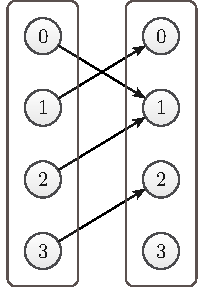
\includegraphics[width=\textwidth]{figures/periodicity_example_a.pdf}
    \end{minipage}
    \hfill
    \begin{minipage}{0.73\textwidth}
      \[
        T(x) \define
        \begin{cases}
          1 &: x \in \set{0,2}{} \\
          0 &: x = 1 \\
          2 &: x = 3
        \end{cases}
        \separate
      % \]
      % \[
        (u_n) =
        \begin{cases}
          \overline{10} &: s_0 \in \set{0,2}{} \\
          \overline{01} &: s_0 = 1 \\
          2\overline{10} &: s_0 = 3
        \end{cases}
      \]
    \end{minipage}
    \medskip
    \par
    \noindent
    The first example shows a transition function which is not bijective but does not map any element of $S$ to itself.
    Hence, in all cases we get a period of $2$.
    The transient varies between $1$ and $2$ and depends on the seed value.

    \medskip
    \begin{minipage}{0.2\textwidth}
      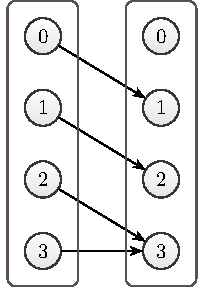
\includegraphics[width=\textwidth]{figures/periodicity_example_b.pdf}
    \end{minipage}
    \hfill
    \begin{minipage}{0.73\textwidth}
      \[
        T(x) \define
        \begin{cases}
          x + 1 &: x < 3 \\
          3 &: x = 3
        \end{cases}
      % \]
      % \[
      \separate
        (u_n) =
        \begin{cases}
          12\overline{3} &: s_0 = 0 \\
          2\overline{3} &: s_0 = 1 \\
          \overline{3} &: s_0 \geq 2 \\
        \end{cases}
      \]
    \end{minipage}
    \medskip

    \noindent
    In the second example, again a non-bijective transition function is used.
    This time the value $3$ is mapped to itself and as a consequence the period for all possible sequences is $1$.
    As before, the transient varies with respect to the seed value.

    \medskip
    \begin{minipage}{0.2\textwidth}
      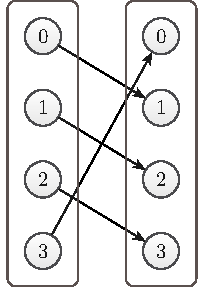
\includegraphics[width=\textwidth]{figures/periodicity_example_c.pdf}
    \end{minipage}
    \hfill
    \begin{minipage}{0.73\textwidth}
      \[
        T(x) \define x + 1 \mod 4
      % \]
      % \[
      \separate
        (u_n) =
        \begin{cases}
          \overline{1230} &: s_0 = 0 \\
          \overline{2301} &: s_0 = 1 \\
          \overline{3012} &: s_0 = 2 \\
          \overline{0123} &: s_0 = 3
        \end{cases}
      \]
    \end{minipage}
    \medskip

    \noindent
    In the third example, a bijective transition function is used.
    The period is maximized and reaches the number of states.
    In all cases the transient is $1$ and as a result all sequences are periodic.

    \medskip
    \begin{minipage}{0.2\textwidth}
      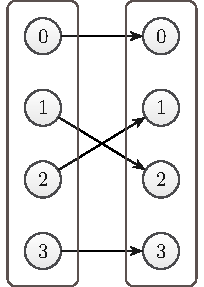
\includegraphics[width=\textwidth]{figures/periodicity_example_d.pdf}
    \end{minipage}
    \hfill
    \begin{minipage}{0.73\textwidth}
      \[
        T(x) \define
        \begin{cases}
          x &: x \in \set{0,3}{} \\
          2 &: x = 1 \\
          1 &: x = 2
        \end{cases}
      % \]
      % \[
      \separate
        (u_n) =
        \begin{cases}
          \overline{0} &: s_0 = 0 \\
          \overline{21} &: s_0 = 1 \\
          \overline{12} &: s_0 = 2 \\
          \overline{3} &: s_0 = 3
        \end{cases}
      \]
    \end{minipage}
    \medskip

    \noindent
    The last example shows again a bijective transition function $T$.
    The transient is again always $1$ and all possible pseudorandom sequences are purely periodic.
    But this time, $T$ maps the values $0$ and $3$ to themselves.
    Hence, the period becomes dependent on the initial value and differs between the smallest possible value $1$ and $2$.\\
    The periodic behavior of pseudorandom sequences greatly constrains the possible randomness of a PRNG.
    Especially for simulations, using a PRNG which is repeating itself while in use introduces unwanted regularities resulting in an incorrect output.
    As a consequence, developers of PRNGs try to construct a large period by adjusting the number of states and the transition function.
    For example, the MT19937 is a PRNG with an extremely large period of $2^{19937}-1$ if not used with a seed value of zero \autocite{matsumoto1998}.
    The use of a bijective transition function is not enough to ensure the maximal period.
    Values that are mapped to themselves result in the smallest possible period even if the transient of the sequence could be large.
    Especially for linear PRNGs that are mapping $0$ to itself, developers tend to exclude such states from the seeding process to always obtain the maximal period \autocite{marsaglia2003,blackman2019}.
    As a counter-example, the so-called \enquote{Middle Square RNG} which was developed by Von Neumann in the early days of computer science should be named \autocites[\ppno~12-15]{kneusel2018}{widynski2019}.
    This PRNG computed the square of its current state and returned the middle digits as next random number.
    It was well known to suffer from the \enquote{zero mechanism} --- once some digits become zero, all following return values would be zero as well \autocites[\ppno~12-15]{kneusel2018}{widynski2019}.
    So besides a large state space and a bijective transition function, the largest possible permutation cycle should be reached when advancing the state of a PRNG.

    \paragraph{Equidistribution}
    Pseudorandom sequences should mimic the behavior of truly random sequences.
    And for that reason, we want them to be uniformly distributed on the set of output values in some sense.
    This property will make it possible to generate every important distribution of random numbers by applying special transformations based on stochastics.
    Such distributions can then be used by Monte Carlo simulations to estimate solutions more efficiently.
    But because we are dealing with actual values instead of random variables, we have to clarify what uniformly distributed means.
    Consequently, we will again rely on probability theory to elaborate on the details without a deeper understanding of randomness \autocite{eisner2019}.
    To be able to always distinct these two different concepts, we will call a sequence of actual values with the desired properties equidistributed.

    \begin{definition}[Equidistributed Sequence]
      Let $U$ be a non-empty, finite set of values and μ be a probability measure on the measurable space $(U,\mathscr{P}(U))$.
      A sequence $(u_n)_{n\in\setNatural}$ in $U$ is equidistributed with respect to μ if for every measurable function $\function{X}{U}{\setReal}$ the following is true.
      \[
        \lim_{n\to\infty} \frac{1}{n} \sum_{k=1}^n X(u_k) = \integral{U}{}{X}{μ}
      \]
      If μ is not specified, we assume it to be the uniform distribution on $U$.
    \end{definition}
    The idea is that every possible output value should essentially be reached the same amount of times when advancing the state.
    For pseudorandom sequences generated by a non-bijective transition function the transient part should be ignored as it can be seen as non-recurring \enquote{warm-up} time.
    Therefore equidistribution will be evaluated at infinity in the sense of a limit.
    Because we wanted to use probability theory to observe randomness, we had to generalize the idea of counting how often different output values would be reached.
    Instead we use arbitrary measurable functions as observables to estimate their expectation value with respect to the given sequence and to compare it to their actual expectation value \autocite{eisner2019}.
    Please note that for our needs we have chosen a finite set of elements to simplify the definition of equidistribution.
    A more general alternative where $U$ has to be a compact metric space with Borel probability measure μ can be found in \textcite{eisner2019}.
    Here, measurable functions are interchanged with continuous functions.
    Because of this, we can further simplify the right-hand side of the definition.
    \[
      \integral{U}{}{X}{μ} = \expect X = \sum_{u\in U} f(u) μ(\set{u}{})
    \]
    To make sure the generalization is working properly, we proof the following lemma which states that, while observing pseudorandom sequences, the relative frequency in one period of an arbitrary element must be given by its probability.

    \begin{lemma}[Equidistributed Pseudorandom Sequences]
      Let $\mathscr{G}\define (S,T,U,G)$ be a PRNG with $s_0\in S$ as its seed value and $(u_n)_{n\in\setNatural}$ the respective pseudorandom sequence with transient τ and period ρ.
      Furthermore, let μ be a probability measure on $(U,\mathscr{P}(U))$.
      Then the following statements are equivalent.
      \begin{enumerate}[label=(\roman*)]
        \item $(u_n)$ is equidistributed with respect to μ.
        \item For all $u\in U$ the following is true.
          \[
            \frac{1}{ρ} \cdot \#\set{n\in\setNatural}{τ\leq n < ρ+τ, u_n = u} = μ(\set{u}{})
          \]
      \end{enumerate}
    \end{lemma}
    \begin{proof}
      Because $U$ is a finite set, every measurable function $\function{X}{U}{\setReal}$ can be described as a linear combination of characteristic functions with respect to some real coefficients $α_u$ for all $u \in U$ in the following way.
      \[
        X = \sum_{u\in U} α_u \mathds{1}_{\set{u}{}}
      \]
      Hence, without loss of generality, it suffices to take only characteristic functions into account.
      Let $u\in U$ be arbitrary.
      The right-hand side of the definition will then result in the following.
      \[
        \integral{U}{}{\mathds{1}_{\set{u}{}}}{μ} = μ(\set{u}{})
      \]
      Applying the characteristic function together with the properties of a periodic sequence to the left-hand side of the definition, looks as follows.
      \[
        \begin{aligned}
          \lim_{n\to\infty} \frac{1}{n} \sum_{k=1}^n \mathds{1}_{\set{u}{}}(u_k)
          &= \lim_{n\to\infty} \frac{1}{n} \sum_{k=1}^{τ-1} \mathds{1}_{\set{u}{}}(u_k) + \lim_{n\to\infty} \frac{1}{n}\sum_{k=τ}^{τ+n-1} \mathds{1}_{\set{u}{}}(u_k) \\
          &= \frac{1}{ρ} \sum_{k=τ}^{τ+ρ-1} \mathds{1}_{\set{u}{}}(u_k) \\
          &= \frac{1}{ρ} \cdot \#\set{n\in\setNatural}{τ\leq n < ρ+τ, u_n = u}
        \end{aligned}
      \]
      This shows the desired equivalence and proofs the lemma.
    \end{proof}
    Based on this lemma, it directly follows that for equidistributed, pseudorandom sequences with a maximal period the number of different states has to be a multiple of the number of output values.

    \begin{corollary}[Equidistributed Pseudorandom Sequence with Maximal Period]
      Let $\mathscr{G}\define (S,T,U,G)$ be a PRNG with $s_0\in S$ as its initial state and $(u_n)_{n\in\setNatural}$ the respective pseudorandom sequence.
      If $(u_n)$ is equidistributed and periodic with maximal period $\# S$ then the following is true.
      \[
        \exists k\in\setNatural:\quad \# S = k \cdot \# U
      \]
    \end{corollary}
    % The given definition can be directly applied to PRNGs.

    % \begin{definition}[Equidistribution]
    %   Let $\mathscr{G}\define (S,T,U,G)$ be a PRNG and $S_0 \subset S$ a set of seeds.
    %   $\mathscr{G}$ is said to be equidistributed with respect to $S_0$ if for all seeds $s_0 \in S_0$ the respective pseudorandom sequence is equidistributed.
    % \end{definition}
    % A PRNG is called equidistributed if every possible pseudorandom sequence is equidistributed.

    \paragraph{Multidimensional Equidistribution}
    Typical Monte-Carlo Simulations need to construct random vectors.
    Due to the shown dependence of successive values of pseudorandom sequence not every PRNG is suited for such applications.
    The following property quantifies in how many dimensions a PRNG can be used.

    \begin{definition}[Multidimensional Equidistribution]
      Let $\mathscr{G}\define (S,T,U,G)$ be a PRNG and $S_0 \subset S$ a set of seeds and $k \in \setNatural$.
      \[
        v_n \define (u_i)_{i\in I_n}
        \separate
        I_n \define \set{τ + (n-1)k + p}{p\in\setNatural, p \leq k}
      \]
      $\mathscr{G}$ is said to be $k$-dimensional equidistributed with respect to $S_0$ if for all $τ\in\setNatural_0$ and seeds $s_0\in S_0$ the respective $k$-dimensional, pseudorandom vector sequence $(v_n)$ is equidistributed on $U^k$.
    \end{definition}
    For some typical examples we refer to images and references.

    \paragraph{Linearity}
    \begin{definition}[Linearity]

    \end{definition}

    \paragraph{Discrepancy}

    \paragraph{Predictability and Security}


    \subsubsection{Implementation-Specific Performance}
    \paragraph{Seekability}


    \subsubsection{Analyzation}
    visualization, proof, experiments, benchmarks (runtime), test suites, code analyzation

    statistical quality and performance vs implementation quality and performance

    Visualizations: randograms 2d and 3d, histograms, simulation plots and images

    Period and Uniformity, Empirical Testing, predictability and Security, Speed, Memory Size, Code Size, Output Range, Seekability, multiple streams, k-dimensional equidistribution, theoretical support, repeatability, portability, ease of implementation
    % subsubsection random_and_pseudorandom_number_generators (end)

    \subsubsection{Examples}
    % \subsubsection{Linear Congruential Generator} % (fold)
    % \label{ssub:linear_congruential_generator}
      \begin{definition}[Linear Congruential Generator]
        Let $m\in\setNatural$ with $m\geq 2$ and $a,c\in\setInteger_m$.
        We define the PRNG $\mathrm{LCG}(m,a,c) \define (S,T,U,G)$
        \[
          S \define U \define \setInteger_m
          \separate
          G \define \identity_{\setInteger_m}
        \]
        \[
          \function{T}{S}{S}
          \separate
          T(x) \define a x + c
        \]
        Multiplication and addition are understood in the sense of $\setInteger_m$.
        We call $\mathrm{LCG}(m,a,c)$ the linear congruential generator with modulus $m$, multiplier $a$ and increment $c$.
      \end{definition}
    % subsubsection linear_congruential_generator (end)

    % \subsubsection{Mersenne Twister} % (fold)
    % \label{ssub:mersenne_twister}
      \begin{definition}[Mersenne Twister]
        Let $w, n, m\in \setNatural$ and $r\in\setNatural_0$ with $m \leq n$ and $r < w$.
        Further, let $a,b,c \in \setInteger_2^w$ and $u,s,t,l \in \setInteger_w$.
        Then the Mersenne Twister $\mathrm{MT}(w,n,m,r,a,b,c,u,s,t,l)\define (S,T,U,G)$ is defined as a PRNG in the following way.
        \[
          S \define \setInteger_n \times \setInteger_2^{w\times n}
          \separate
          U \define \setInteger_2^w
        \]
        \[
          \function{T}{S}{S}
        \]
        \[
          \forall i\in\setInteger_{n-1}: T(i, x) \define (i + 1, x)
        \]
        \[
          T(n-1, x) \define (0, y)
        \]
        \begin{align*}
          \forall i\in\setInteger_{n-m}: y_i &\define x_{m+i} \oplus \roundBrackets{x_i^u \middle\vert x_{i+1}^l}A \\
          \forall i\in\setInteger_{m-1} + (n-m): y_i &\define y_{i-(n-m)} \oplus \roundBrackets{x_i^u \middle\vert x_{i+1}^l}A \\
          y_{n-1} &\define y_{m-1} \oplus \roundBrackets{x^u_{n-1} \middle\vert y_0^l}A
        \end{align*}
        \[
          xA \define
          \begin{cases}
            x \gg 1 &: x_0 = 0 \\
            (x \gg 1) \oplus a &: x_0 = 1
          \end{cases}
        \]
        \[
          f_1(x) \define x \oplus (x \gg u)
        \]
        \[
          f_2(x) \define x \oplus ((x \ll s) \odot b)
        \]
        \[
          f_3(x) \define x \oplus ((x \ll t) \odot c)
        \]
        \[
          f_4(x) \define x \oplus (x \gg l)
        \]
        \[
          \function{G}{S}{U}
          \separate
          G(i,x) \define f_4 \circ f_3 \circ f_2 \circ f_1(x_i)
        \]
      \end{definition}
    % subsubsection mersenne_twister (end)

    % \subsubsection{Permuted Congruential Generator} % (fold)
    % \label{ssub:permuted_congruential_generator}
      \begin{definition}[Permuted Congruential Generator]
        Given $\mathscr{G}\define \mathrm{LCG}(b,a,c)$ with transition function $T$.
        Let $t\in\setInteger_{b}$ and $\function{f_c}{\setInteger_{2^{b-t}}}{\setInteger_{2^{b-t}}}$ be a permutation for all $c \in \setInteger_{2^t}$.
        \[
          S \define \setInteger_{2^b}
          \separate
          U \define \setInteger_{2^{b-t}}
        \]
        \[
          G \define π_2 \circ f_* \circ \mathrm{split}_t
        \]
        \[
          f_*(a,b) \define (a,f_a(b))
        \]
        $\mathrm{PCG}(\mathscr{G},t,\set{f_c}{c\in\setInteger_{2^t}}) \define (S,T,U,G)$
      \end{definition}
    % subsubsection permuted_congruential_generator (end)

    % \subsubsection{Xorshift and Variants} % (fold)
    % \label{ssub:xorshift_and_variants}
      \begin{definition}[Xoroshiro128+]
        Let $a,b,c \in \setInteger_{64}$.
        \[
          S \define \setInteger_{2^{64}}^2
          \separate
          U \define \setInteger_{2^{64}}
        \]
        \[
          T(x,y) \define (x \circlearrowleft a \oplus f(x,y) \oplus (f(x,y) \leftarrow b), f(x,y) \circlearrowleft c)
        \]
        \[
          f(x,y) \define x \oplus y
        \]
        \[
          G(x,y) \define x + y
        \]
      \end{definition}
    % subsubsection xorshift_and_variants (end)

    % \subsubsection{Middle Square Weyl Sequence RNG} % (fold)
    % \label{ssub:middle_square_weyl_sequence_rng}
      \begin{definition}[Middle Square Weyl Sequence RNG]
        Let $s\in\setInteger_{2^{64}}$ be an odd constant.
        The middle square Weyl sequence RNG $\mathrm{MSWS}(s)\define(S,T,U,G)$ is defined as a PRNG in the following way.
        \[
          S \define \setInteger_{2^{64}}^2
          \separate
          U \define \setInteger_{2^{32}}
        \]
        \[
          \function{T}{S}{S}
          \separate
          T(w,x) = (w+s, f(x^2 + w + s))
        \]
        \[
          \function{f}{\setInteger_{2^{64}}}{\setInteger_{2^{64}}}
          \separate
          f(x) \define (x \gg 32) \mathrm{or} (x \ll 32)
        \]
        \[
          \function{G}{S}{U}
          \separate
          G(w,x) \define x \mod 2^{32}
        \]
      \end{definition}
    % subsubsection middle_square_weyl_sequence_rng (end)
  % subsection pseudorandom_number_generators (end)

  \subsection{Simulation in Physics and Mathematics} % (fold)
  \label{sub:simulation_in_physics_and_mathematics}
    \subsubsection{Mathematical and Physical Preliminaries} % (fold)
    \label{ssub:mathematical_and_physical_preliminaries}

    % subsubsection mathematical_and_physical_preliminaries (end)

    \subsubsection{Baseline Model Problems} % (fold)
    \label{ssub:baseline_model_problems}

    % subsubsection baseline_model_problems (end)
  % subsection simulation_in_physics_and_mathematics (end)

  \subsection{SIMD-Capable Processors} % (fold)
  \label{sub:simd-capable_processors}
    \subsubsection{Architecture of Modern Central Processing Units} % (fold)
    \label{ssub:architecture_of_modern_central_processing_units}

    % subsubsection architecture_of_modern_central_processing_units (end)

    \subsubsection{SIMD Instruction Sets and Efficiency} % (fold)
    \label{ssub:simd_instruction_sets_and_efficiency}

    % subsubsection simd_instruction_sets_and_efficiency (end)

    \subsubsection{SSE, AVX, AVX512} % (fold)
    \label{ssub:sse_avx_avx512}

    % subsubsection sse_avx_avx512 (end)
  % subsection simd-capable_processors (end)

  \subsection{Summary} % (fold)
  \label{sub:summary}

    \textcite{volchan2002,kneusel2018}
    \autocites[1]{volchan2002}[2]{kneusel2018}

  % subsection summary (end)
% section background (end)
\end{document}